\chapter{Proposta Conceitual}

Esta seção apresenta uma proposta de utilização de \textit{templates} hierárquicos para criar e manipular questões de programação. A ideia inclui o emprego de inteligência artificial generativa como ferramenta complementar, responsável por sugerir variações criativas no \textit{template} base, tais como modificações de contexto, acréscimo de novos cenários e introdução de pontos de variação. Além disso, a IA generativa também oferece suporte no fornecimento de \textit{feedback} imediato ao estudante após a submissão da resposta, apontando erros, sugerindo melhorias e apresentando explicações detalhadas sobre o problema e possíveis soluções. 

\subsection{Geral para o Específico}
A geração automática de questões segue um processo hierárquico que se inicia em tópicos mais amplos e evolui até questões específicas. Em primeiro lugar, definem-se os tópicos da ementa, que correspondem a áreas ou domínios do conhecimento a serem avaliados (por exemplo, Estruturas de Repetição, Estruturas de Decisão, Matrizes, Funções). Esses tópicos abrangem conteúdos extensos do currículo e orientam a elaboração de modelos cognitivos. Na etapa seguinte, tais modelos cognitivos são convertidos em \textit{templates} (ou modelos de questões), que servirão de base para a geração das questões específicas. Essa abordagem reflete a metodologia recomendada para a criação de questões baseadas em \textit{templates}. 

\begin{figure}[ht]
	\centering
	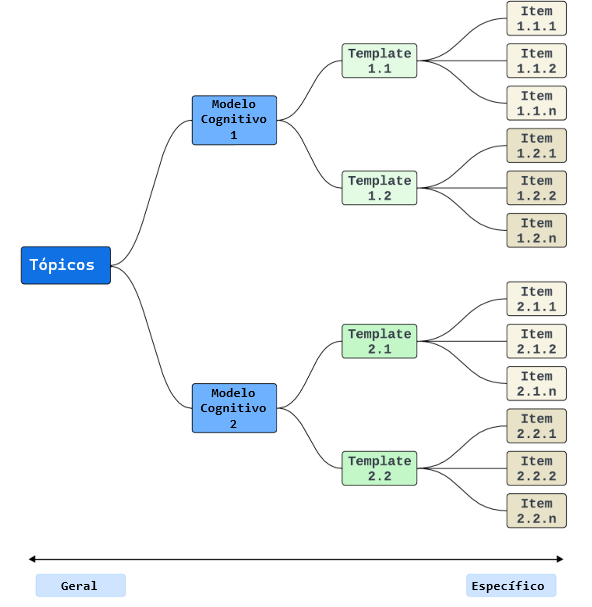
\includegraphics[width=14cm]{./imagens/capitulo5/geral-especifico-com-topicos}
	\caption{Geral para o específico, (adaptado, \cite{hendrickson2010}) }
	\label{fig:geral-to-specif}
\end{figure}